\documentclass[12pt, a4papre]{article}
\usepackage[catalan]{babel}
\usepackage[unicode]{hyperref}
\usepackage[dvipsnames]{xcolor}
\usepackage{amsmath}
\usepackage{amssymb}
\usepackage{amsthm}
\usepackage{xifthen}
\usepackage{siunitx}
\usepackage{xcolor}
\usepackage{float}
\usepackage{listings}
\usepackage{setspace}
\usepackage{subcaption}
\usepackage{graphicx}
\usepackage{tikz,lipsum,lmodern}
\usepackage[most]{tcolorbox}
\usepackage{fancyvrb}
\usepackage{circuitikz}
\usepackage{indentfirst}
\usepackage{verbatimbox}
\usepackage{verbatim}
\usepackage[utf8]{inputenc}
\definecolor{mygreen}{RGB}{28,172,0} % color values Red, Green, Blue
\definecolor{mylilas}{RGB}{170,55,241}
\graphicspath{ {./dades/} }


%% 
%% AMPL definition (c) 2007 Mirko Maischberger 
%% 
\lstdefinelanguage{AMPL}{ 
alsoletter={.},% 
morekeywords={Current,IN,INOUT,Infinity,Initial,LOCAL,OUT,all,binary,% 
by,check,complements,contains,default,dimen,div,else,environ,exists,% 
forall,if,in,integer,less,logical,max,min,option,setof,shell_exitcode,% 
slve_exitcode,solve_message,solve_result,solve_result_num,suffix,sum,% 
symbolic,table,then,union,until,while,within,from,to,obj,% 
cross,diff,symdiff,inter,% 
and,not,or,prod,product},%keywords 
morekeywords=[2]{abs,acos,acosh,alias,asin,asinh,atan,atan2,atanh,ceil,% 
ctime,cos,exp,floor,log,log10,max,min,precision,round,sin,sinh,sqrt,tan,% 
tanh,time,trunc,% 
Beta,Cauchy,Exponential,Gamma,Irand224,Normal,Normal101,Poisson,% 
Uniform,Uniform01,% 
num,num0,ichar,char,length,substr,sprintf,match,sub,gsub,% 
card,next,nextw,prev,prevw,first,last,member,ord,ord0,arity,indexarity,% 
interval,integer,ordered,circular,coeff,cover},%functions 
morekeywords=[3]{set,param,var,arc,minimize,maximize,subject to,% 
node,subjto,s.t.},%declarations 
morekeywords=[4]{call,cd,check,close,commands,data,delete,display,drop,end,% 
environ,exit,expand,fix,include,let,load,model,objective,option,print,% 
printf,problem,purge,quit,read,read table,redeclare,reload,remove,reset,% 
restore,shell,show,solexpand,solution,solve,update,unfix,unload,write,% 
write table,xref},%commands 
sensitive=true,% 
morecomment=[s]{/}{/},% 
morecomment=[l]\#,% 
morestring=[d]",% 
morestring=[d]'% 
}[keywords,comments,strings]% 


\newcommand{\norm}[1]{\lvert #1 \rvert}

\hypersetup{
    colorlinks = true,
    linkcolor = blue
}

\author{}
\title{El problema de la braquistòcrona usant tècniques d'optimització}
\date{24 de Desembre del 2020}

\begin{document}
	\maketitle
	\begin{center}
		\begin{tabular}{ |c | c |}
			\hline
			\textbf{Nom} 		& \textbf{DNI}		\\ \hline
			Rubén Aciego 		&48038376R 		\\ 
			Daniel Vilardell 		&48109585W 		\\
			\hline
		\end{tabular}
	\end{center}
	\tableofcontents
	
	\newpage
	\section{Formulació matematica del problema}
	
	La formulació matematica es ben senzilla, el que hem de minimitzar es el temps que tarda en arribar a $(a, b)$ tenint en compte que $t = \frac{d}{v}$ i que si discretitzem $x$ i $y$  la $d_i=\sqrt{(x_i - x_{i - 1})^2 + (y_i - y_{i - 1})^2}$ ens donaria la distancia entre dos punts de la funció $(x_{i - 1}, y_{i - 1})$ i $(x_i, y_i)$. La velositat en un fragment de distancia es calcularia de la forma que ens han proposat al enunciat, es a dir $v_ =\sqrt{2gy_i}$. Aixi doncs el problema a resoldre es el següent:
	
	\begin{align*}
	P \colon	 min\quad \sum_{i = 1}^n& \frac{\sqrt{(x_i - x_{i - 1})^2 + (y_i - y_{i - 1})^2}} {\sqrt{2gy_i}}\\	
			&x_0 = 0 \qquad
			y_0 = 0\\
			&x_n = a \qquad
			y_n = b\\
	\end{align*}
	
	Tenint en compte però que multiplicar per $\frac{1}{\sqrt{2g}}$ no variarà el resultat, ja que es una constant, podem formular el problema de la següent forma.
	
	\begin{align*}
	P \colon	 min\quad \sum_{i = 1}^n& \sqrt{\frac{(x_i - x_{i - 1})^2 + (y_i - y_{i - 1})^2} {y_i}}\\	
			&x_0 = 0 \qquad
			y_0 = 0\\
			&x_n = a \qquad
			y_n = b\\
	\end{align*}
	
	\newpage
	\section{Codis i gràfiques}
	
	\subsection{Fitxer .run gloval}
	\lstinputlisting[language=AMPL, basicstyle=\tiny]{practica3.run}
	
	\subsection{Fitxers .mod}
	\subsubsection{Part a}
	\lstinputlisting[language=AMPL, basicstyle=\tiny]{practica3_a.mod}
	\subsubsection{Part b}
	\lstinputlisting[language=AMPL, basicstyle=\tiny]{practica3_b.mod}
	\subsubsection{Part c}
	\lstinputlisting[language=AMPL, basicstyle=\tiny]{practica3.mod}
	
	\subsection{Fitxers .dat}
	\subsubsection{Part a}
	\lstinputlisting[language=AMPL, basicstyle=\tiny]{practica3_a.dat}
	\subsubsection{Part b}
	\lstinputlisting[language=AMPL, basicstyle=\tiny]{practica3_b.dat}
	\subsubsection{Part c}
	\lstinputlisting[language=AMPL, basicstyle=\tiny]{practica3.dat}
	
	\subsection{Grafiques}
	\subsubsection{Part a}
	\begin{figure}[H]
		\begin{center}
		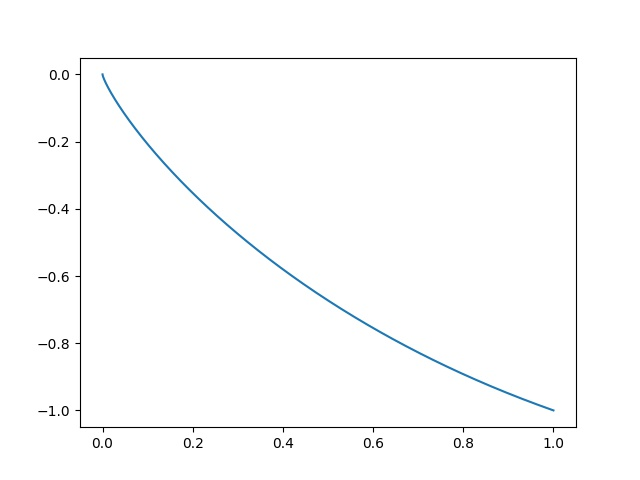
\includegraphics[width=100mm]{modelA500.jpg}
		\end{center}
		\caption{Grafica model A amb $n = 500$}
		
                    \centering
                    \begin{minipage}[b]{0.49\textwidth}
                        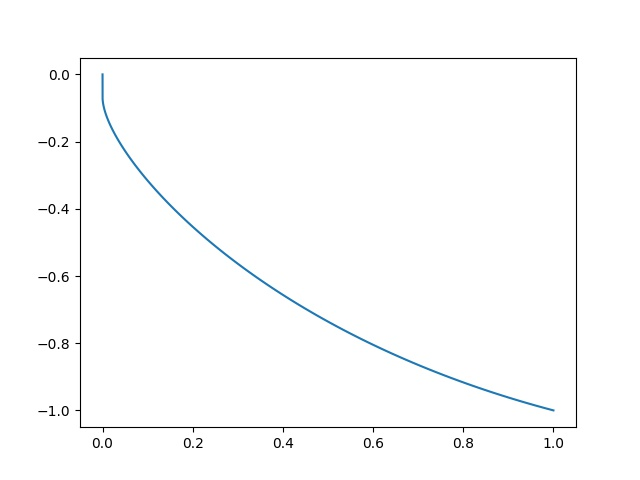
\includegraphics[width=\textwidth]{modelA100.jpg}
                        \caption{\begin{footnotesize} Grafica model A amb $n = 100$ \end{footnotesize}}
                    \end{minipage}
                    \hfill
                    \begin{minipage}[b]{0.49\textwidth}
                        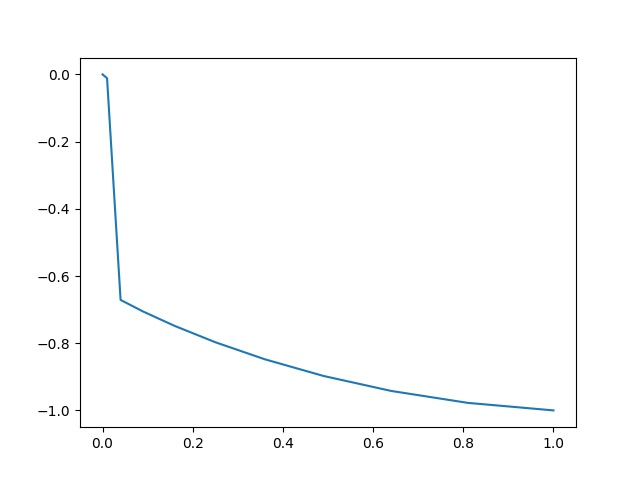
\includegraphics[width=\textwidth]{modelA10.jpg}
                        \caption{\begin{footnotesize} Grafica model A amb $n = 10$ \end{footnotesize}}
                    \end{minipage}
                
	\end{figure}
	
	\subsubsection{Part b}
	
	\begin{figure}[H]
		\begin{center}
		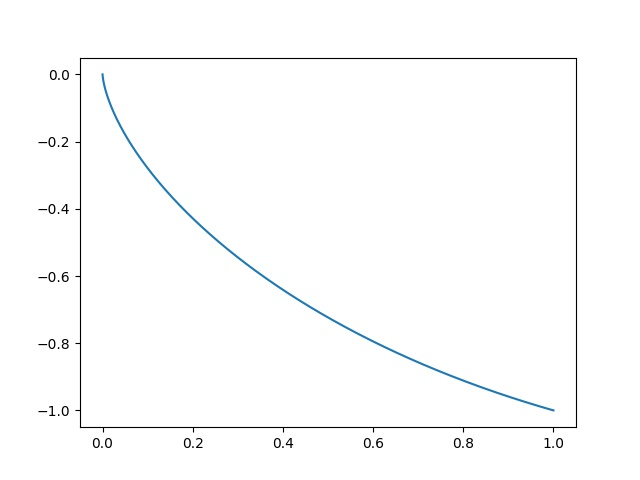
\includegraphics[width=100mm]{modelB500.jpg}
		\end{center}
		\caption{Grafica model B amb $n = 500$}
		
                    \centering
                    \begin{minipage}[b]{0.49\textwidth}
                        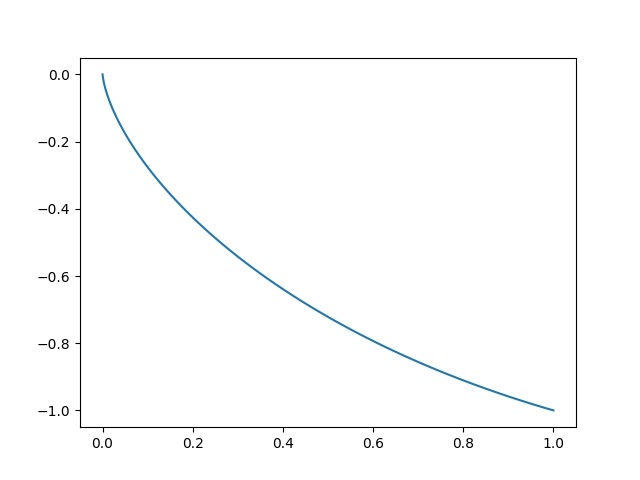
\includegraphics[width=\textwidth]{modelB100.jpg}
                        \caption{\begin{footnotesize} Grafica model B amb $n = 100$ \end{footnotesize}}
                    \end{minipage}
                    \hfill
                    \begin{minipage}[b]{0.49\textwidth}
                        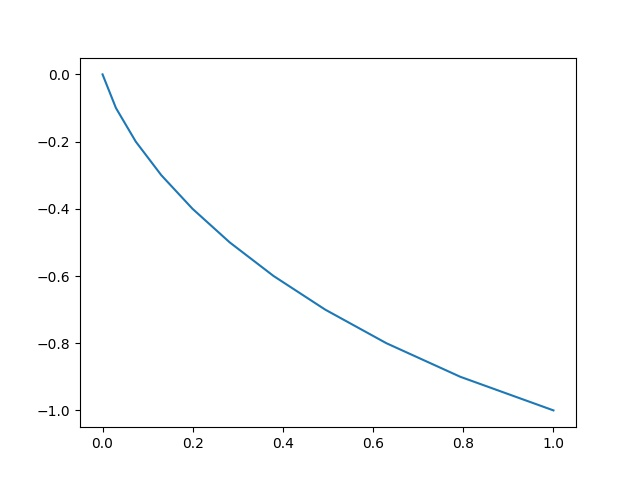
\includegraphics[width=\textwidth]{modelB10.jpg}
                        \caption{\begin{footnotesize} Grafica model B amb $n = 10$ \end{footnotesize}}
                    \end{minipage}
                
	\end{figure}

	\subsubsection{Part c}
	
	\begin{figure}[H]
		\begin{center}
		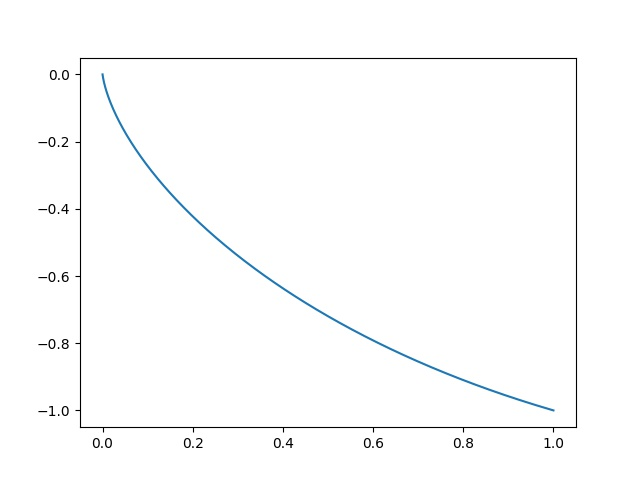
\includegraphics[width=100mm]{modelC500.jpg}
		\end{center}
		\caption{Grafica model C amb $n = 500$}
		
                    \centering
                    \begin{minipage}[b]{0.49\textwidth}
                        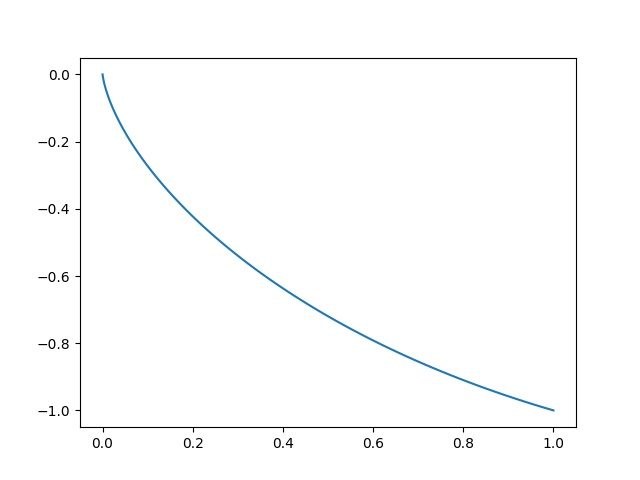
\includegraphics[width=\textwidth]{modelC100.jpg}
                        \caption{\begin{footnotesize} Grafica model C amb $n = 100$ \end{footnotesize}}
                    \end{minipage}
                    \hfill
                    \begin{minipage}[b]{0.49\textwidth}
                        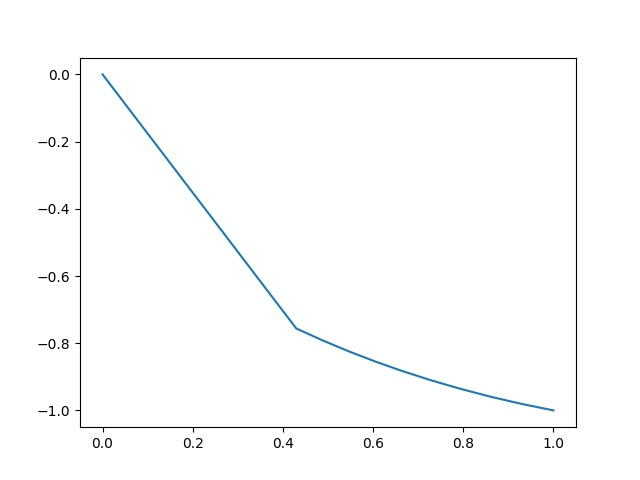
\includegraphics[width=\textwidth]{modelC10.jpg}
                        \caption{\begin{footnotesize} Grafica model C amb $n = 10$ \end{footnotesize}}
                    \end{minipage}
                
	\end{figure}
	
	\newpage
	\section{Demostració de que el model B es un problema convex}
	
	Per tal de demostrar això veurem que el determinant de la Hessiana es semidefinit positiu. Com que nomes te com a variable les x, calculem la segona derivada de $f(x) = \sum_{i = 1}^n \sqrt{\frac{(x_i - x_{i - 1})^2 + (y_i - y_{i - 1})^2} {y_i}}$. Com que y es un vector constant calcular aquesta matriu hessiana no serà massa complicat. Per linealitat de les derivades, si demostrem que la hessiana de $g(x) =  \sqrt{\frac{(x_i - x_{i - 1})^2 + (y_i - y_{i - 1})^2} {y_i}}$ per tot $i \in (1, n)$ es semidefinida positiva, la hessiana de la funció original serà definida.
	
	\[
	\nabla g(x) =(\frac{x_{i - 1} - x_{i}}{\sqrt{(x_{i} - x_{i - 1})^2 + (y_i - y_{i - 1})^2}}, \frac{x_{i} - x_{i - 1}}{\sqrt{(x_{i} - x_{i - 1})^2 + (y_i - y_{i -1})^2}})
	\]
	
	\[
	\nabla^2 g(x) = 
	\begin{pmatrix}
	\frac{(y_{i} - y_{i - 1})^2}{((x_{i} - x_{i - 1})^2 + (y_i - y_{i - 1})^2)^{\frac{3}{2}}}	& \frac{-(y_{i} - y_{i - 1})^2}{((x_{i} - x_{i - 1})^2 + (y_i - y_{i - 1})^2)^{\frac{3}{2}}}\\
	\frac{-(y_{i} - y_{i - 1})^2}{((x_{i} - x_{i - 1})^2 + (y_i - y_{i - 1})^2)^{\frac{3}{2}}}	& \frac{(y_{i} - y_{i - 1})^2}{((x_{i} - x_{i - 1})^2 + (y_i - y_{i - 1})^2)^{\frac{3}{2}}}
	\end{pmatrix}
	\]
	
	Com que tots els menors de la matriu hessiana son positius, per el criteri de Sylvester podem confirmar que la matriu hessiana es semidefinida positiva i per tant la funció $g(x)$ es convexa. La suma de funcions convexas dona com a resultat una funció convexa i per tant $f(x)$ es convexa. Com que les restriccions també son convexes ja que es tracten de una igualtat en un punt, podem confirmar que el model B del problema es un problema d'optimització convex.



\end{document}
